\section{Rate of Generators Change} %3.5
\label{section3.5}
Generators have a limit on the output power (in MW) and another limit on the rate of change of power (in MW/minute). The rate of change of power is called ramp rate. It expresses how quickly a power plant's power output is changing. 

\begin{equation}
    Rate = \frac{\Delta P}{\Delta t}
\end{equation}


According to National Renewable Energy Lab., Golden, CO (US), \cite{osti_15016292} large thermal units are usually able to ramp around 1\% of their capacity per minute. For instance, if a generator's nominal power is 360 MW, its ramp rate will be 3.6 MW/min or 0.06 MW/sec.\\

In this project, benefiting from \sys{pyramses}~\footnote{\sys{pyramses} is a Python library for \sys{RAMSES} dynamic simulator: \href{https://anaconda.org/apetros/pyramses}{https://anaconda.org/apetros/pyramses}}, it's possible to get generators' power output directly from the simulator. Thus, through the MATLAB \sys{stepinfo}~\footnote{\sys{stepinfo} contains \sys{Rise time}, \sys{settling time}, and other step-response characteristics. Document: \href{https://www.mathworks.com/help/control/ref/stepinfo.html}{https://www.mathworks.com/help/control/ref/stepinfo.html}} module, we can use \sys{Peak} and \sys{PeakTime} to calculate the ramp rate:

\begin{equation}
    Rate = \frac{P_{\sys{peak}} - P_o}{\sys{PeakTime}}
\end{equation}

where $P_o$ is the original power output of a generator when SFC starts (i.e. $P_{t=0}$ when the SFC starts).\\

I have to explain why I don't use \sys{RiseTime} to calculate the ramp rate. It seems like \sys{RiseTime} ensures the rate's reliability from its definition: "Time it takes for the response to rise from 10\% to 90\% of the steady-state response". However, unlike frequency, generators do not have steady-state response ($y_{final}$). Traditionally, we can use the final value of the signal as steady-state response ($y_{final}$). However, in this case, as shown in Figure~\ref{3_5_yfinal1} and in Figure~\ref{3_5_yfinal2}, different tuning results may bring different $y_{final}$. It makes using $y_{final}$ as steady-state response nearly impossible. Choosing \sys{Peak} and \sys{PeakTime} that are not related with steady-state response is necessary.

\begin{figure}[!t]
\center
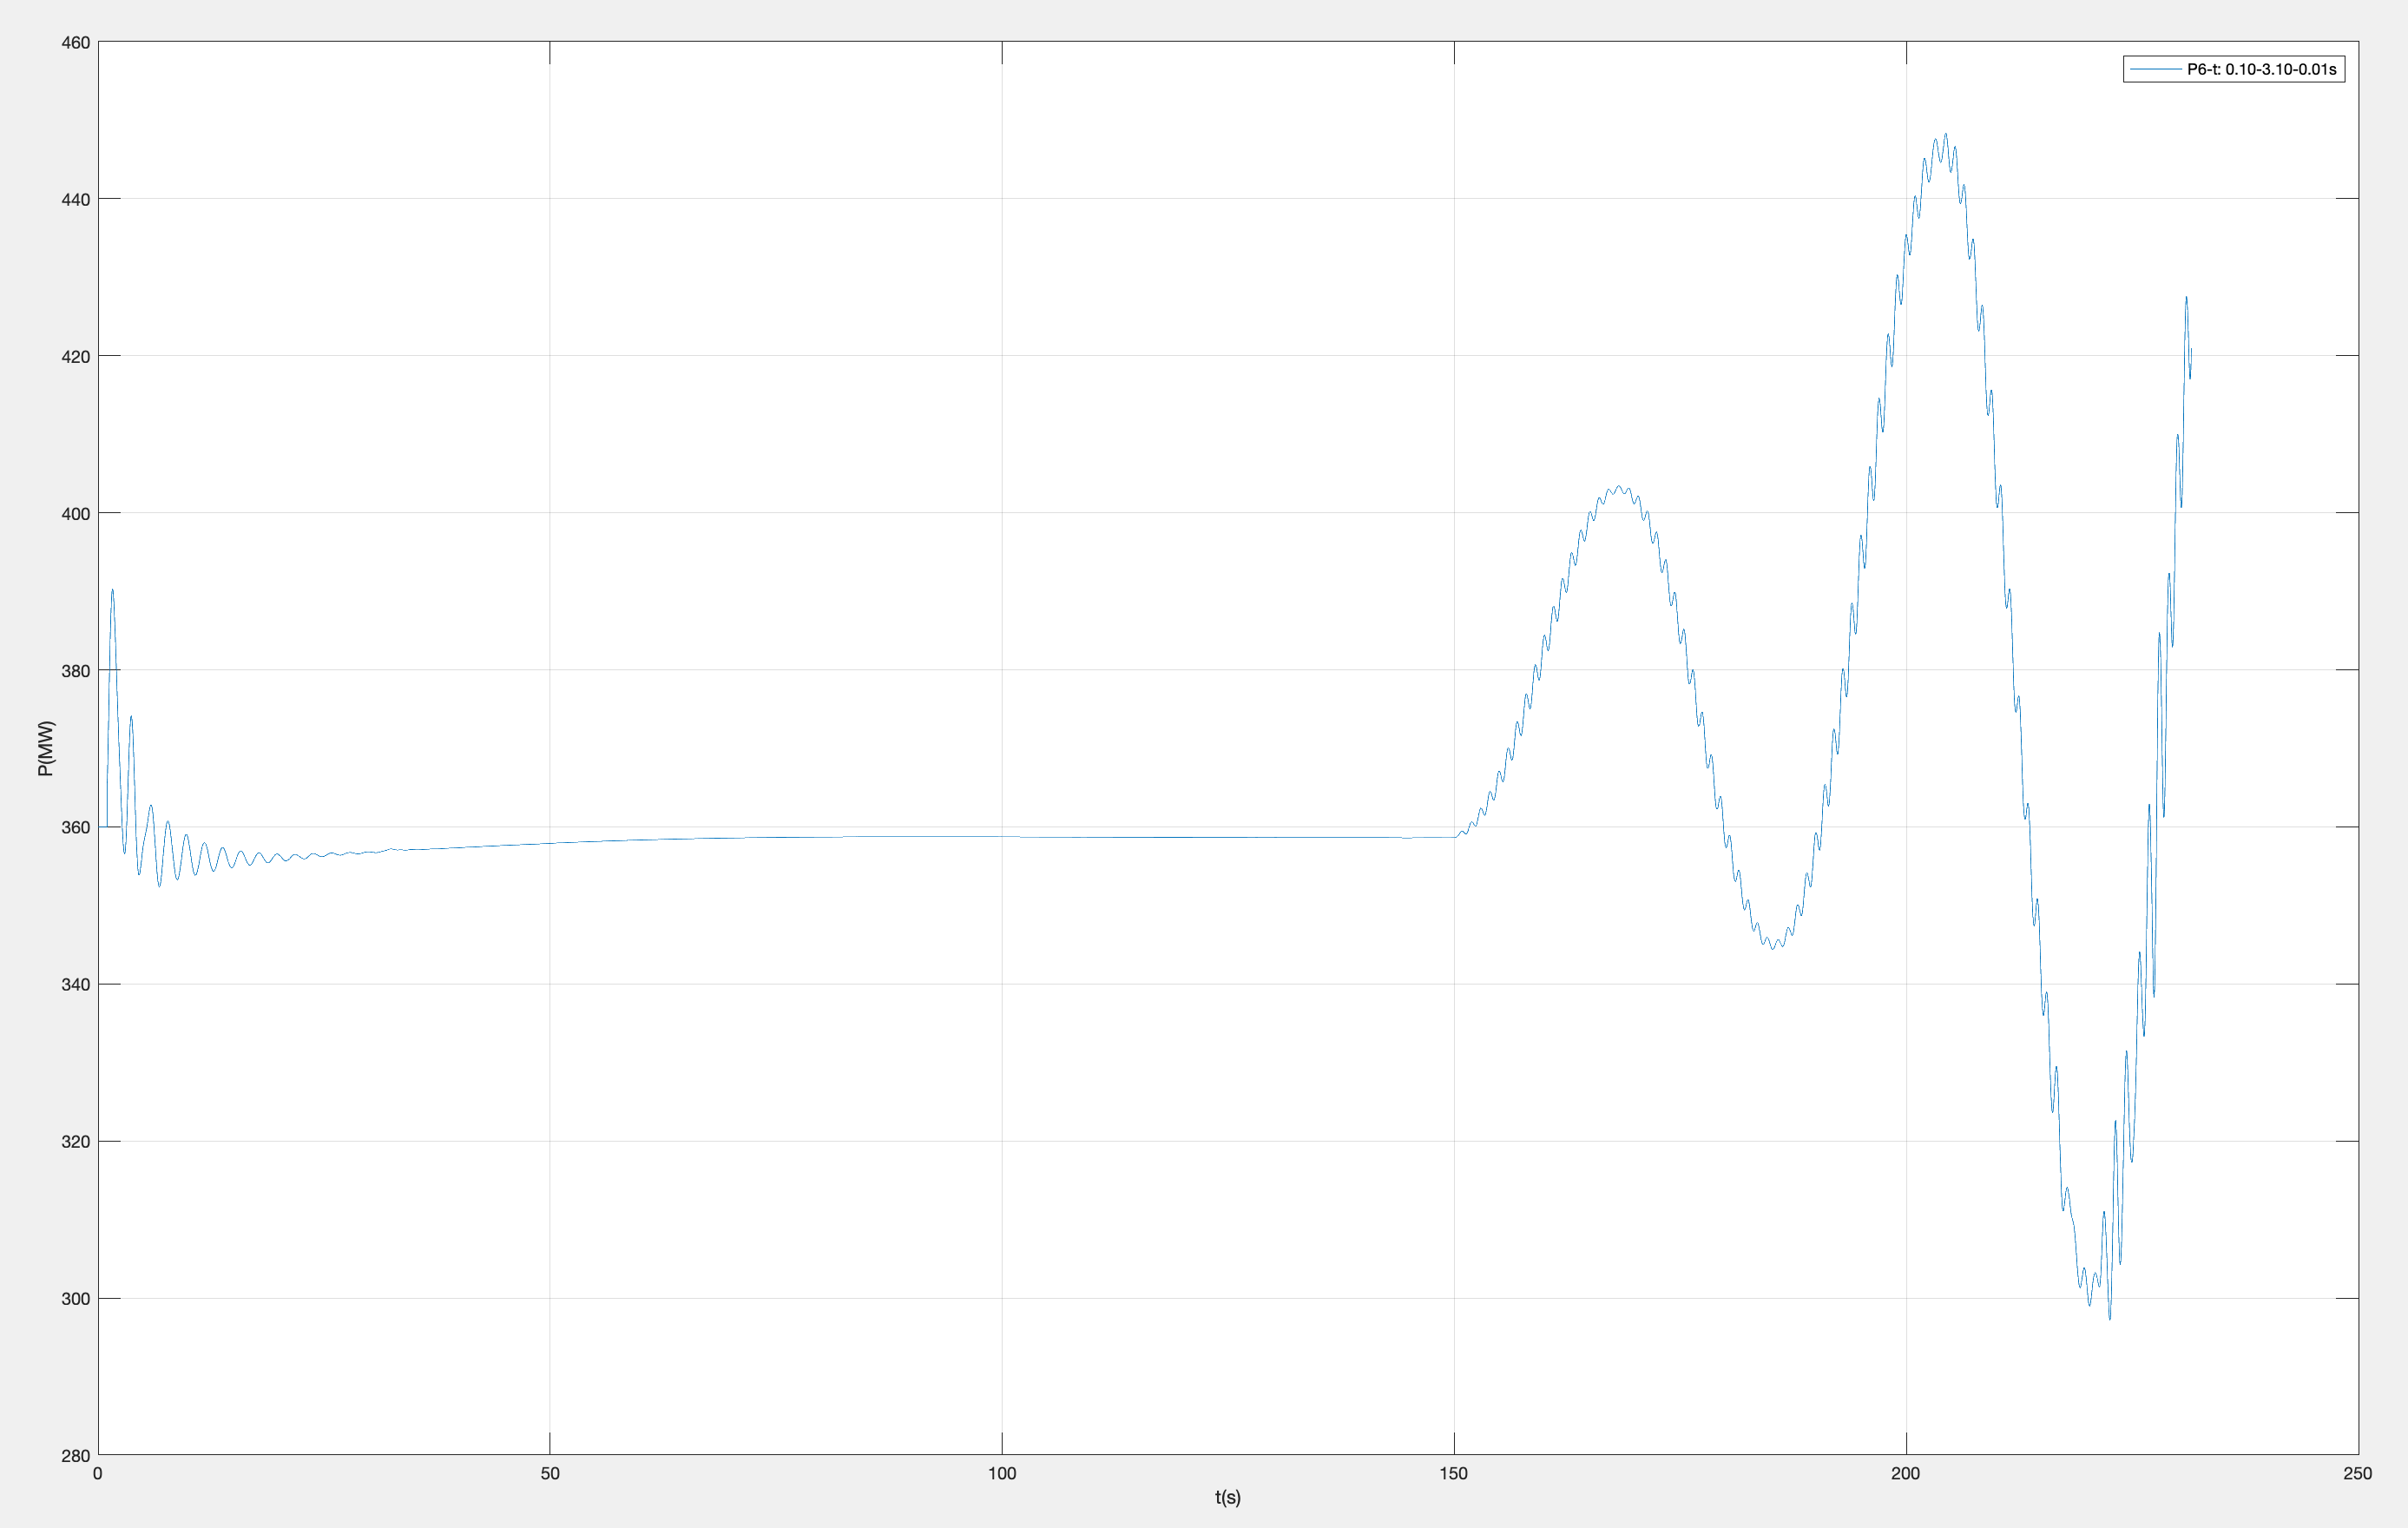
\includegraphics[scale=0.25]{figure/3_5_yfinal1.png}
\caption{g6's power output: kp=0.1, ki=3.1}
\label{3_5_yfinal1}
\end{figure}

\begin{figure}[!t]
\center
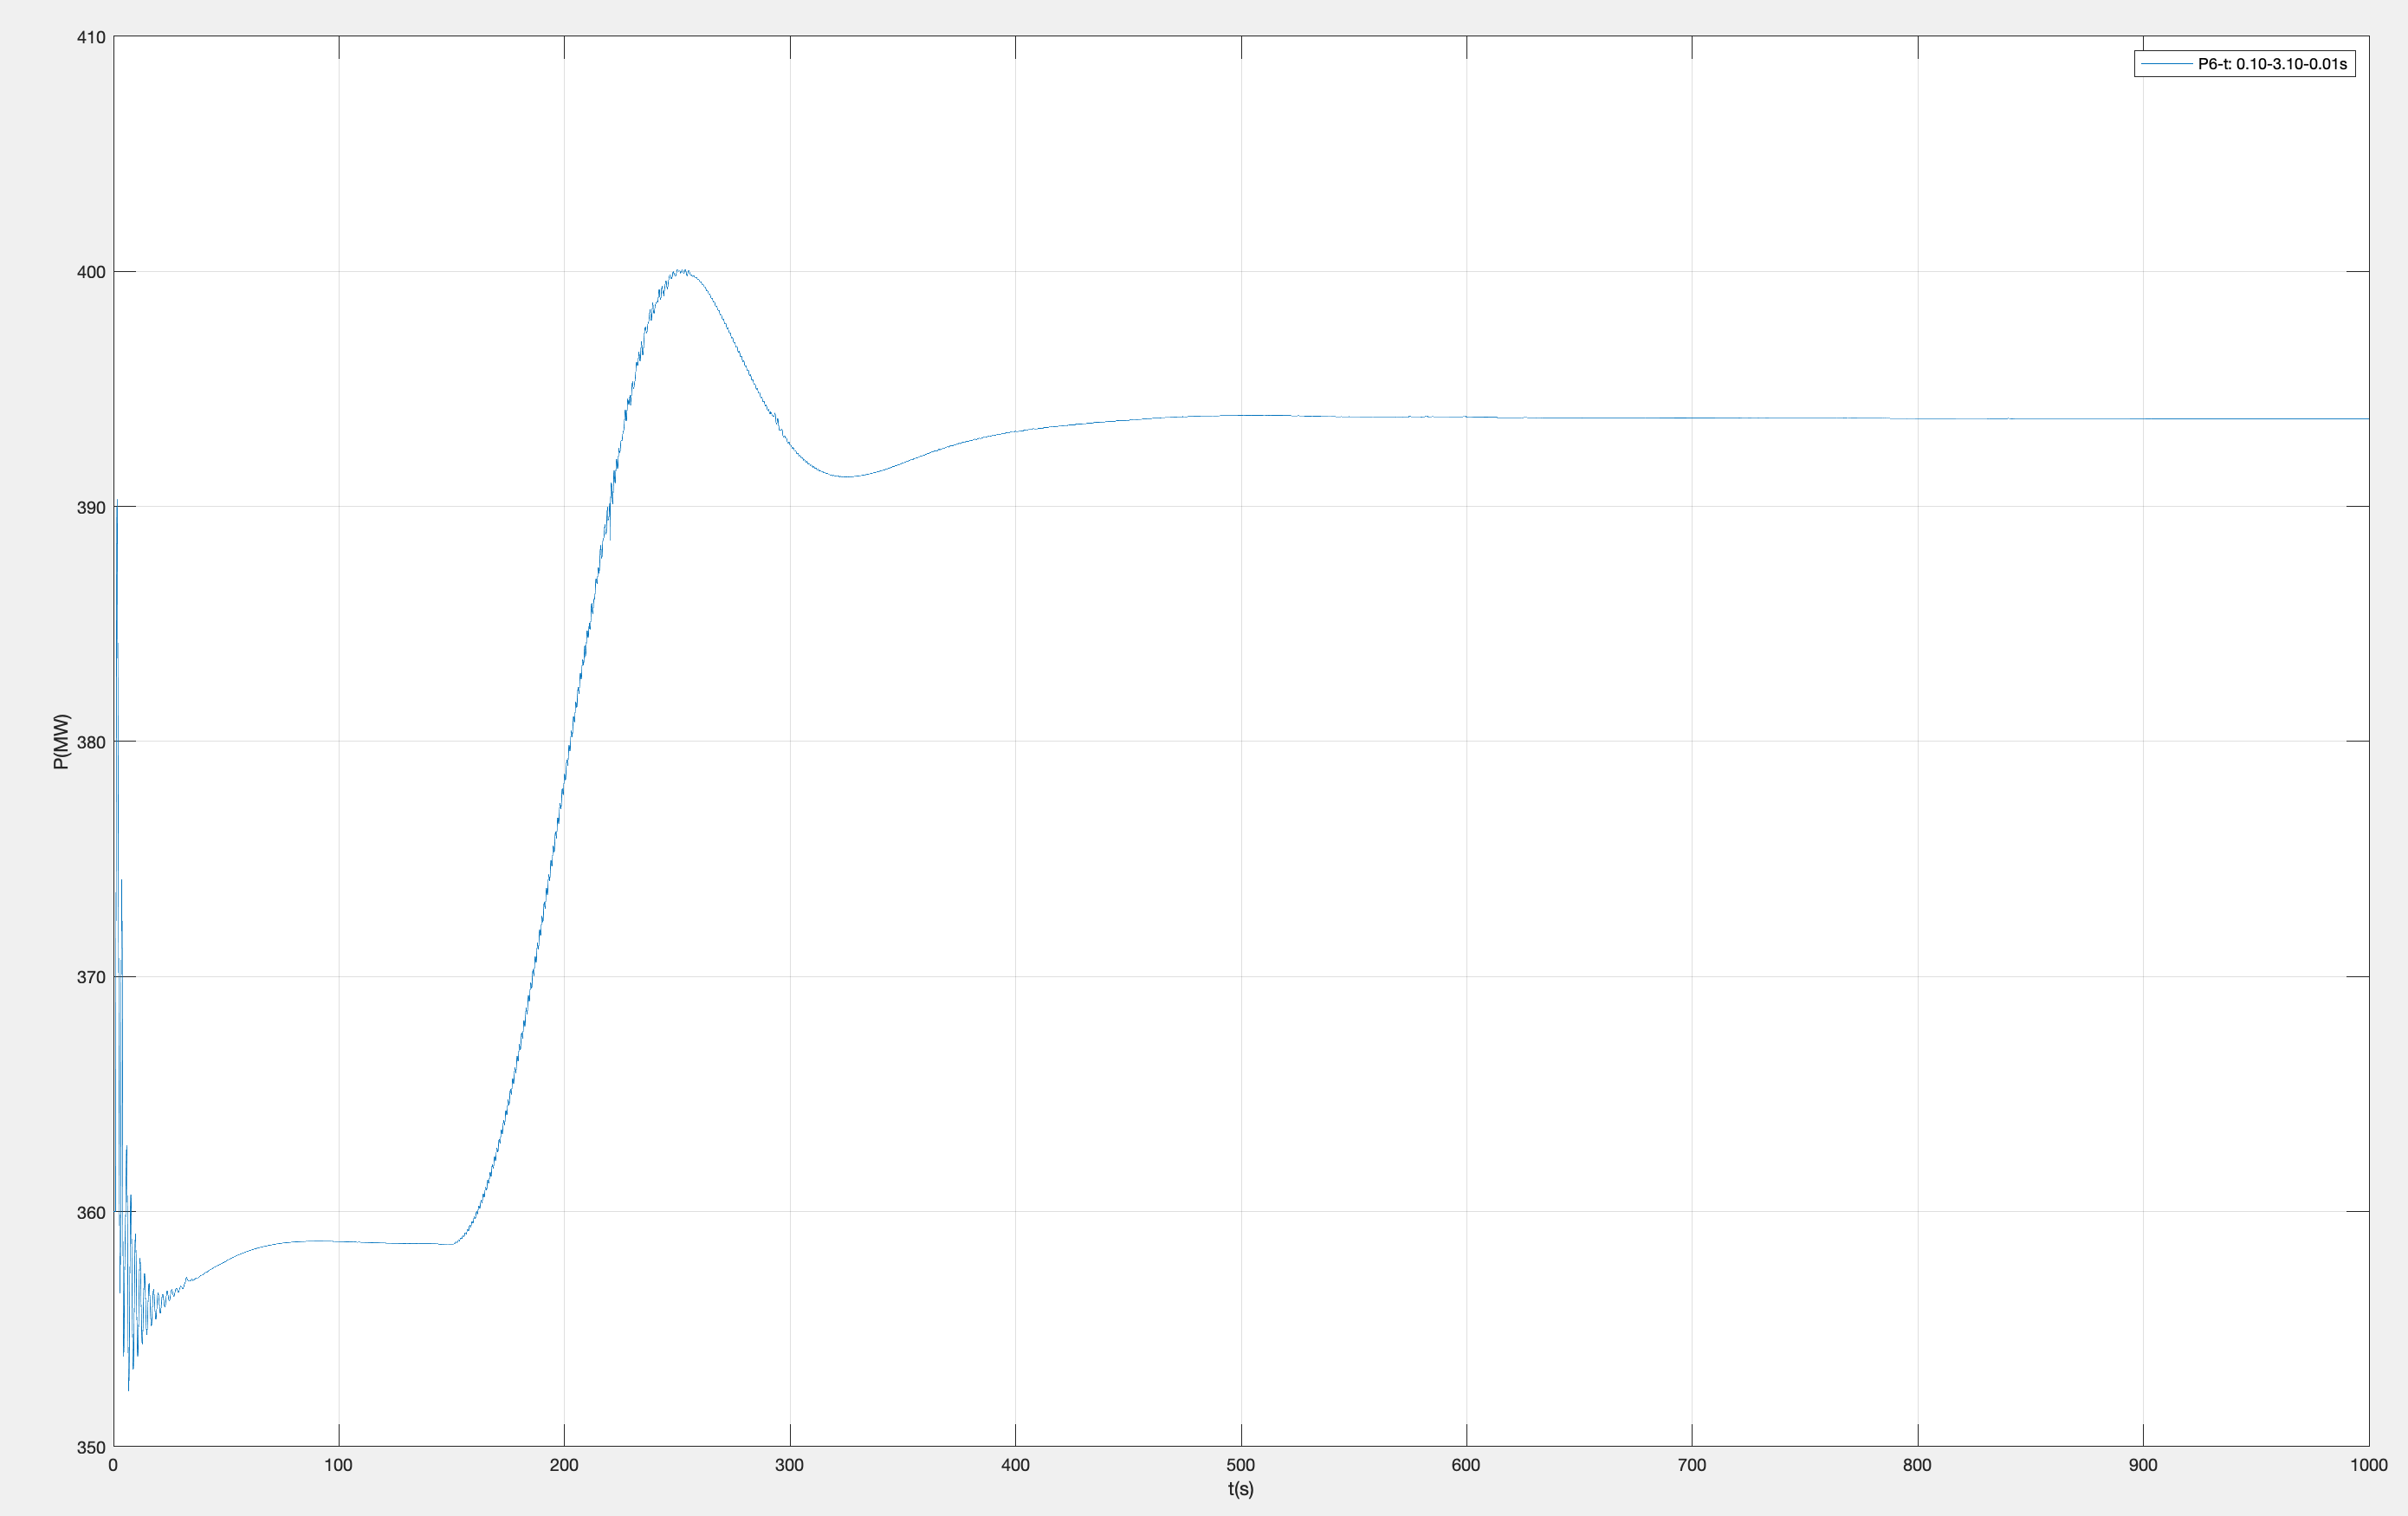
\includegraphics[scale=0.25]{figure/3_5_yfinal2.png}
\caption{g6's power output: kp=0.1, ki=0.1}
\label{3_5_yfinal2}
\end{figure}

